
\subsection{Space Partitioning}

  \begin{figure}[h]
    \begin{center}
      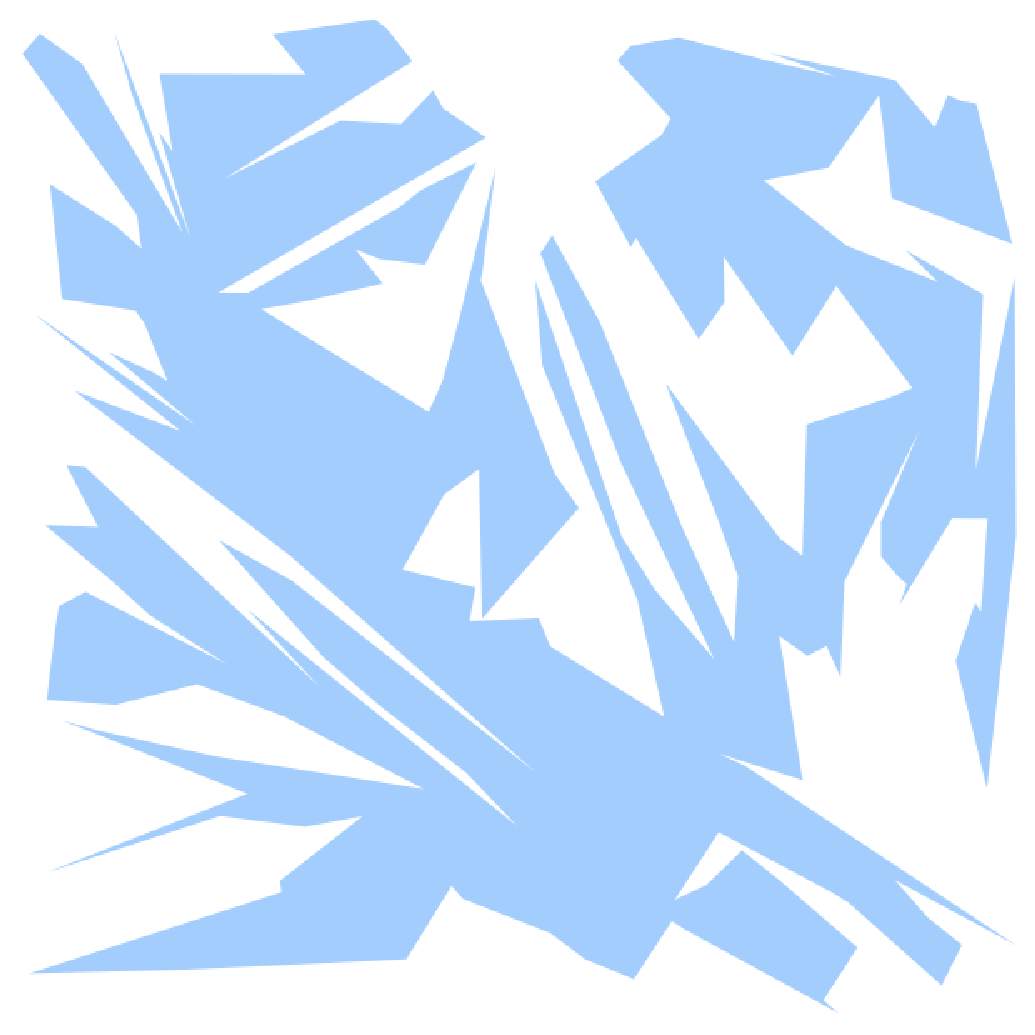
\includegraphics[width=0.3\textwidth]{img/spacepart200.eps}
    \end{center}
    \caption{Polygon mit 200 Punkten (Space Partitioning)}
    \label{fig:space200}
  \end{figure}

  \enquote{Space Partitioning} ist einer der von T. Auer und M. Held 
  in~\cite{held98polygons} beschriebenen Algorithmen zur Generierung von
  einfachen Polygonen.


  Es handelt sich dabei um einen Divide und Conquer Algorithmus, der, wie der
  Name schon suggeriert, im Divide-Schritt eine vorgegebene Punktmenge in
  Partitionen mittels einem Halbebenenschnitts aufteilt, dann rekursiv Polygone
  in diesen Halbebenen erzeugt und im Merge-Schritt diese Polygone in ein
  einfaches gesamt Polygon zusammensetzt.

  \subsubsection{Algorithmus}

    Wie oben schon beschrieben ist \enquote{Space Partitioning} ein 
    Divide \& Conquer
    Algorithmus, der in der Betrachtung und Umsetzung die Allgemeine Lage
    voraussetzt. \\

    \noindent
    Space Partitioning besteht im wesentlichen aus drei Schritten:
    \begin{itemize}
      \item[1.] Die Berechnung einer Geraden $l$, die den Rand der Halbebenen 
            repr"asentiert und somit die Punktmenge in zwei eindeutige 
            Partitionen teilt
      \item[2.] Die rekursive Konstruktion eines linken und rechten 
            Teilpolygons innerhalb der Partitionen
      \item[3.] Die Zusammenf"ugung dieser Teilpolygone zu einem gesamten 
            Polygon
    \end{itemize}

    \noindent
    Bevor die Rekursion im Space Partitioning Algorithmus ausgef"uhrt werden
    kann, muss diese gesondert initialisert werden, in dem wir einmalig zwei
    Punkte aus der Punktmenge zuf"allig ausw"ahlen und die Partition anhand der
    Geraden, die durch diese zwei gew"ahlten Punkte verl"auft, vornehmen. \\
    Der eigentliche Rekursionsschritt braucht dabei diese Anfangs- und
    Endpunkte, um eine neue Partitionsgerade zu konstruieren. \\
    In der Implementierung wurde darauf geachtet, dass die in der Rekursion
    erstellten Teilpolygone die Anfangs- bzw. Endpunkte an erster bzw. letzter
    Position in dem  Polygonzug zu stehen haben - je nachdem, ob es sich um das
    linke oder rechte Teilpolygon handelt -, wodurch der Merge-Schritt nur an
    den Grenzen der Polylines Duplikate entfernen musste, um das Polygon zu
    erstellen. Au"serdem wurde auf eine CCW-Sortierung der Punkte geachtet.

    % Einbauen?
    %Wir k"onnen insgesamt folgende Beobachtung in einer Invariante ausdr"ucken:
    %Der Schnitt der beiden Teilpolygone besitzt nur eine gemeinsame Kante und diese ist genau
    %die Strecke den gegebenen Anfangs- und Endpunkte.

    % TODO:
    % die im Prozess der Konstruktion im Allgemeinen nicht einfach bleiben

\begin{code}[caption={Space Partitioning}, mathescape=true]
choose two random points $s_f$ and $s_l$ and remove them

left, right $\leftarrow$ partition points in the left/right side of the line $l(s_f, s_l)$

leftPolygon $\leftarrow$ Space Partitioning(left, $s_f$, $s_l$)
leftPolygon $\leftarrow$ Space Partitioning(right, $s_f$, $s_l$)

polygon $\leftarrow$ merge(leftPolygon, rightPolygon)
\end{code}

    \noindent

    Der Rekursionsschritt l"auft analog zum Initialierungsschritt ab. Nur das
    hier die Partitionierung mithilfe der Geraden $l$ (siehe Z.
    \ref{lst:space_line}) erfolgt. Diese Gerade $l$ wird durch einen zuf"allig
    gew"ahlten Anfangspunkt auf der Strecke $s_f$, $s_l$ und einem zuf"alligen
    Endpunkt aus der Punktmenge ``points'' definiert.

\begin{code}[caption={Rekursion Space Partitioning}, 
            mathescape=true, escapeinside={@}{@}]
Space Partitioning(points, $s_f$, $s_l$)

  if points only contains $s_f$ and $s_l$
    return line segment $s_f$, $s_l$

  $s$ $\leftarrow$ choose random and remove point in points
  @\label{lst:space_line}@$l$ $\leftarrow$ choose random line through $s$, which intersects the line segment $s_f$, $s_l$

  left, right $\leftarrow$ partition points in the left/right side of the line $l$

  leftPolygon $\leftarrow$ Space Partitioning(left, $s_f$, $s$)
  rightPolygon $\leftarrow$ Space Partitioning(right, $s$, $s_l$)

  polygon $\leftarrow$ merge(leftPolygon, rightPolygon)

  return polygon
\end{code}

  \subsubsection{Laufzeit}

    Die Laufzeitanalyse von \enquote{Space Partitioning} ist analog zur
    Laufzeitanalyse von Quicksort. Sei $n$ die Anzahl der vorgegebenen
    Punktmenge. Nach der Rekursionsbaum Analysemethode werden in jeder
    Rekursionsebene  h"ochstens $\bigO(n)$ Operationen ausgef"uhrt (Die
    Punktmenge wird komplett unter den Rekursionaufrufen einer Rekursionsebene
    aufgeteilt). Wodurch die Laufzeit sich nur nach der Rekursionstiefe richtet.
    Bei halbwegs gleicher Aufteilung der Partitionen sind nur $\bigO(\log n)$
    Rekursionsebenen, im worst-case $\bigO(n)$ hingegen n"otig.
    \\ Damit hat \enquote{Space Partitioning} eine worst-case Laufzeit von
    $\bigO(n^2)$, aber in vielen F"allen eine sehr viele bessere $\bigO(n \log
    n)$ Laufzeit.

  \subsubsection{Eigenschaften}

    Aufgrund des einfachen Divide \& Conquer Ansatzes und ausschlie"slichen
    Verwendung von Basis-Operationen, wie z.B. eines Orientierungstests, ist
    \enquote{Space Partitioning} der schnellste implementierte Algorithmus dieses
    Projekts. Wodurch \enquote{Space Partitioning} sich f"ur Testpolygone mit gro"sen
    Punktmengen (100.000 Punkte in weniger als 10s) anbietet. Leider ist ``Space
    Partitioning'' nach T.Auer und M. Held~\cite{held98polygons} nicht
    inclusive,  dennoch geben sie in ihrem Paper an, dass bei 100.000
    Durchl"aufen mit 10 Punkten ungef"ahr 10-20\% der generierten Polygone
    Duplikate von bereits generierten waren. Bei 100 Punkten und 100.000
    Durchl"aufen wurde kein Polygon mehrfach erzeugt. Wodurch es, nach ihrere
    Einsch"atzung, bei gro"sen Punktmengen unwahrscheinlich ist, dass Polygone
    mehrfach generiert werden. Au"serdem konnten sie bei ihrerer Datenanalyse
    feststellen, dass man nicht erwarten sollte, dass die erzeugten Polygone
    gleichverteilt auftreten.

